\documentclass[
%handout,
%draft,
compress]
{beamer}


\defbeamertemplate{section page}{mine}[1][]{%
  \begin{centering}
    {\usebeamerfont{section name}\usebeamercolor[fg]{section name}#1}
    \vskip1em\par
    \begin{beamercolorbox}[sep=12pt,center]{part title}
      \usebeamerfont{section title}\insertsection\par
    \end{beamercolorbox}
  \end{centering}
}
\setbeamertemplate{section page}[mine][]


\usetheme[authorwidth=.20,titlewidth=.50,datewidth=.30,section=true,subsection=true,]{Lund}
\setbeamertemplate{navigation symbols}{}
\usefonttheme[onlymath]{serif}
% automatic table of contents at every section
%\AtBeginSection[]{\frame{\tableofcontents[currentsection]}}
%\usepackage{pdfsync}
\usepackage[utf8x]{inputenc}
\usepackage{tikz}
\SetUnicodeOption{mathletters}
\usepackage{verbatim}
\hypersetup{ % information in the PDF file.
  pdftitle={Catch and throw\\Ball and Beam},%
  pdfauthor={Mattias Fält, Lucas Jimbergsson,\\Erik Nossborn, Iulia Stoica},
%  pdfsubject={Advanced Mathematics},
%  pdfkeywords={groups, triangles, algebras}
}

\title[Catch and Throw]{Catch and throw\\Ball and Beam}
\author[]{Mattias Fält, Lucas Jimbergsson,\\Erik Nossborn, Iulia Stoica\\\vspace{1em}Supervisor -- Karl-Erik Årz\'{e}n}

%\date{2013-09-01}
\begin{document}
\frame{\titlepage}

\section*{Outline}

<<<<<<< HEAD
\frame{\partpage}
=======
%\part{Main Talk}
%\frame{\partpage}
>>>>>>> 4ec0fd49cd8b27dbbd5894a1b280b2b187a20a08

\frame
{
  \frametitle{Outline}
  \tableofcontents%[part=1]%,pausesections]%,shadesubsections]
}

\section{Introduction/problem}
\frame{\sectionpage}
\begin{frame}
\frametitle{Problem formulation}
\begin{itemize}
\item test
\end{itemize}
\end{frame}


\begin{frame}
\frametitle{Difficulties}

\end{frame}

\section{Overall approach}
\frame{\sectionpage}
\begin{frame}
\frametitle{Initial idea}
\begin{itemize}
\item Model the system
\item Find throw equations
\item Calculate trajectories
\item Stabilize with PID/LQG
\end{itemize}
\end{frame}

\begin{frame}

\frametitle{Initial idea}
\begin{columns}
\column{150pt}
\[
\begin{pmatrix}\dot{x}_{1}\\
\dot{x}_{2}\\
\dot{x}_{3}\\
\dot{x}_{4}
\end{pmatrix}=\begin{pmatrix}x_{2}\\
\frac{5}{7}\left(-g\sin(x_{3})+x_{1}x_{4}^{2}\right)\\
x_{4}\\
\frac{1}{J_B}(mgx_{1}\cos(x_3)+\frac{x_3}{J_B}+k_{u})
\end{pmatrix}
\]
\begin{figure}
\centering
\scalebox{0.5}{\begin{tikzpicture}[scale=1.5]
\usetikzlibrary{patterns,snakes}
\definecolor{Darkgreen}{rgb}{0,0.4,0}
\tikzstyle{brace} = [decorate, decoration={brace, amplitude=5pt}]

\node[inner sep=0] (v0) at (0,0) {};
\node[inner sep=0] (v2) at (2,0.5) {};
\node[inner sep=0] (v1) at (-1,-0.25) {};

\draw[color=red]  (v1) edge (v2);

\node (v3) at (8,-2) {};
\node (v4) at (0,-2) {};
\node (v5) at (8,0) {};

\draw[ball color=blue] (2,0.6) circle (.1);

\draw[dashed,->] (v2) -- (4,1) node[pos=1,above] {$\dot{x}$};
\draw[dashed] (v0) -- (v5) {};
\draw[dashed] (v0) -- (v4) {};
\draw[brace] (v0) -- (v2) node[pos=0.5,above,yshift=6] {$l=x$};
\draw[brace] (v3) -- (v4) node[pos=0.5,below,yshift=-6] {$d_x$};
\draw[brace] (v5) -- (v3)  node[pos=0.5,right,xshift=5] {$d_y$};

 \draw[color=green] plot[smooth] coordinates {(v2) (4,0.6) (6,0) (8,-2)};
 
 
\node at (1.3,0.17) {$\phi$};

\path[clip] (2,0.5) -- (0,0) -- (2,0);
\node[circle,draw=Darkgreen, minimum size=90pt] at (0,0) (circ) {};

\end{tikzpicture}}
\end{figure}
\column{150pt}
\[
\dot{x}=\left(d_{x}-l\cos(\phi)\right)\frac{\sqrt{g}}{\sqrt{2\cos(\phi)\left(d_{y}\cos(\phi)+d_{x}\sin(\phi)\right)}}.
\]
\end{columns}
\end{frame}

\begin{frame}
\frametitle{Final solution -- Heuristic approach}

\end{frame}

\begin{frame}
\frametitle{Solutions to difficulties}

\end{frame}

\section{Controller structure}
\frame{\sectionpage}
\begin{frame}
%\frametitle{}
\centering
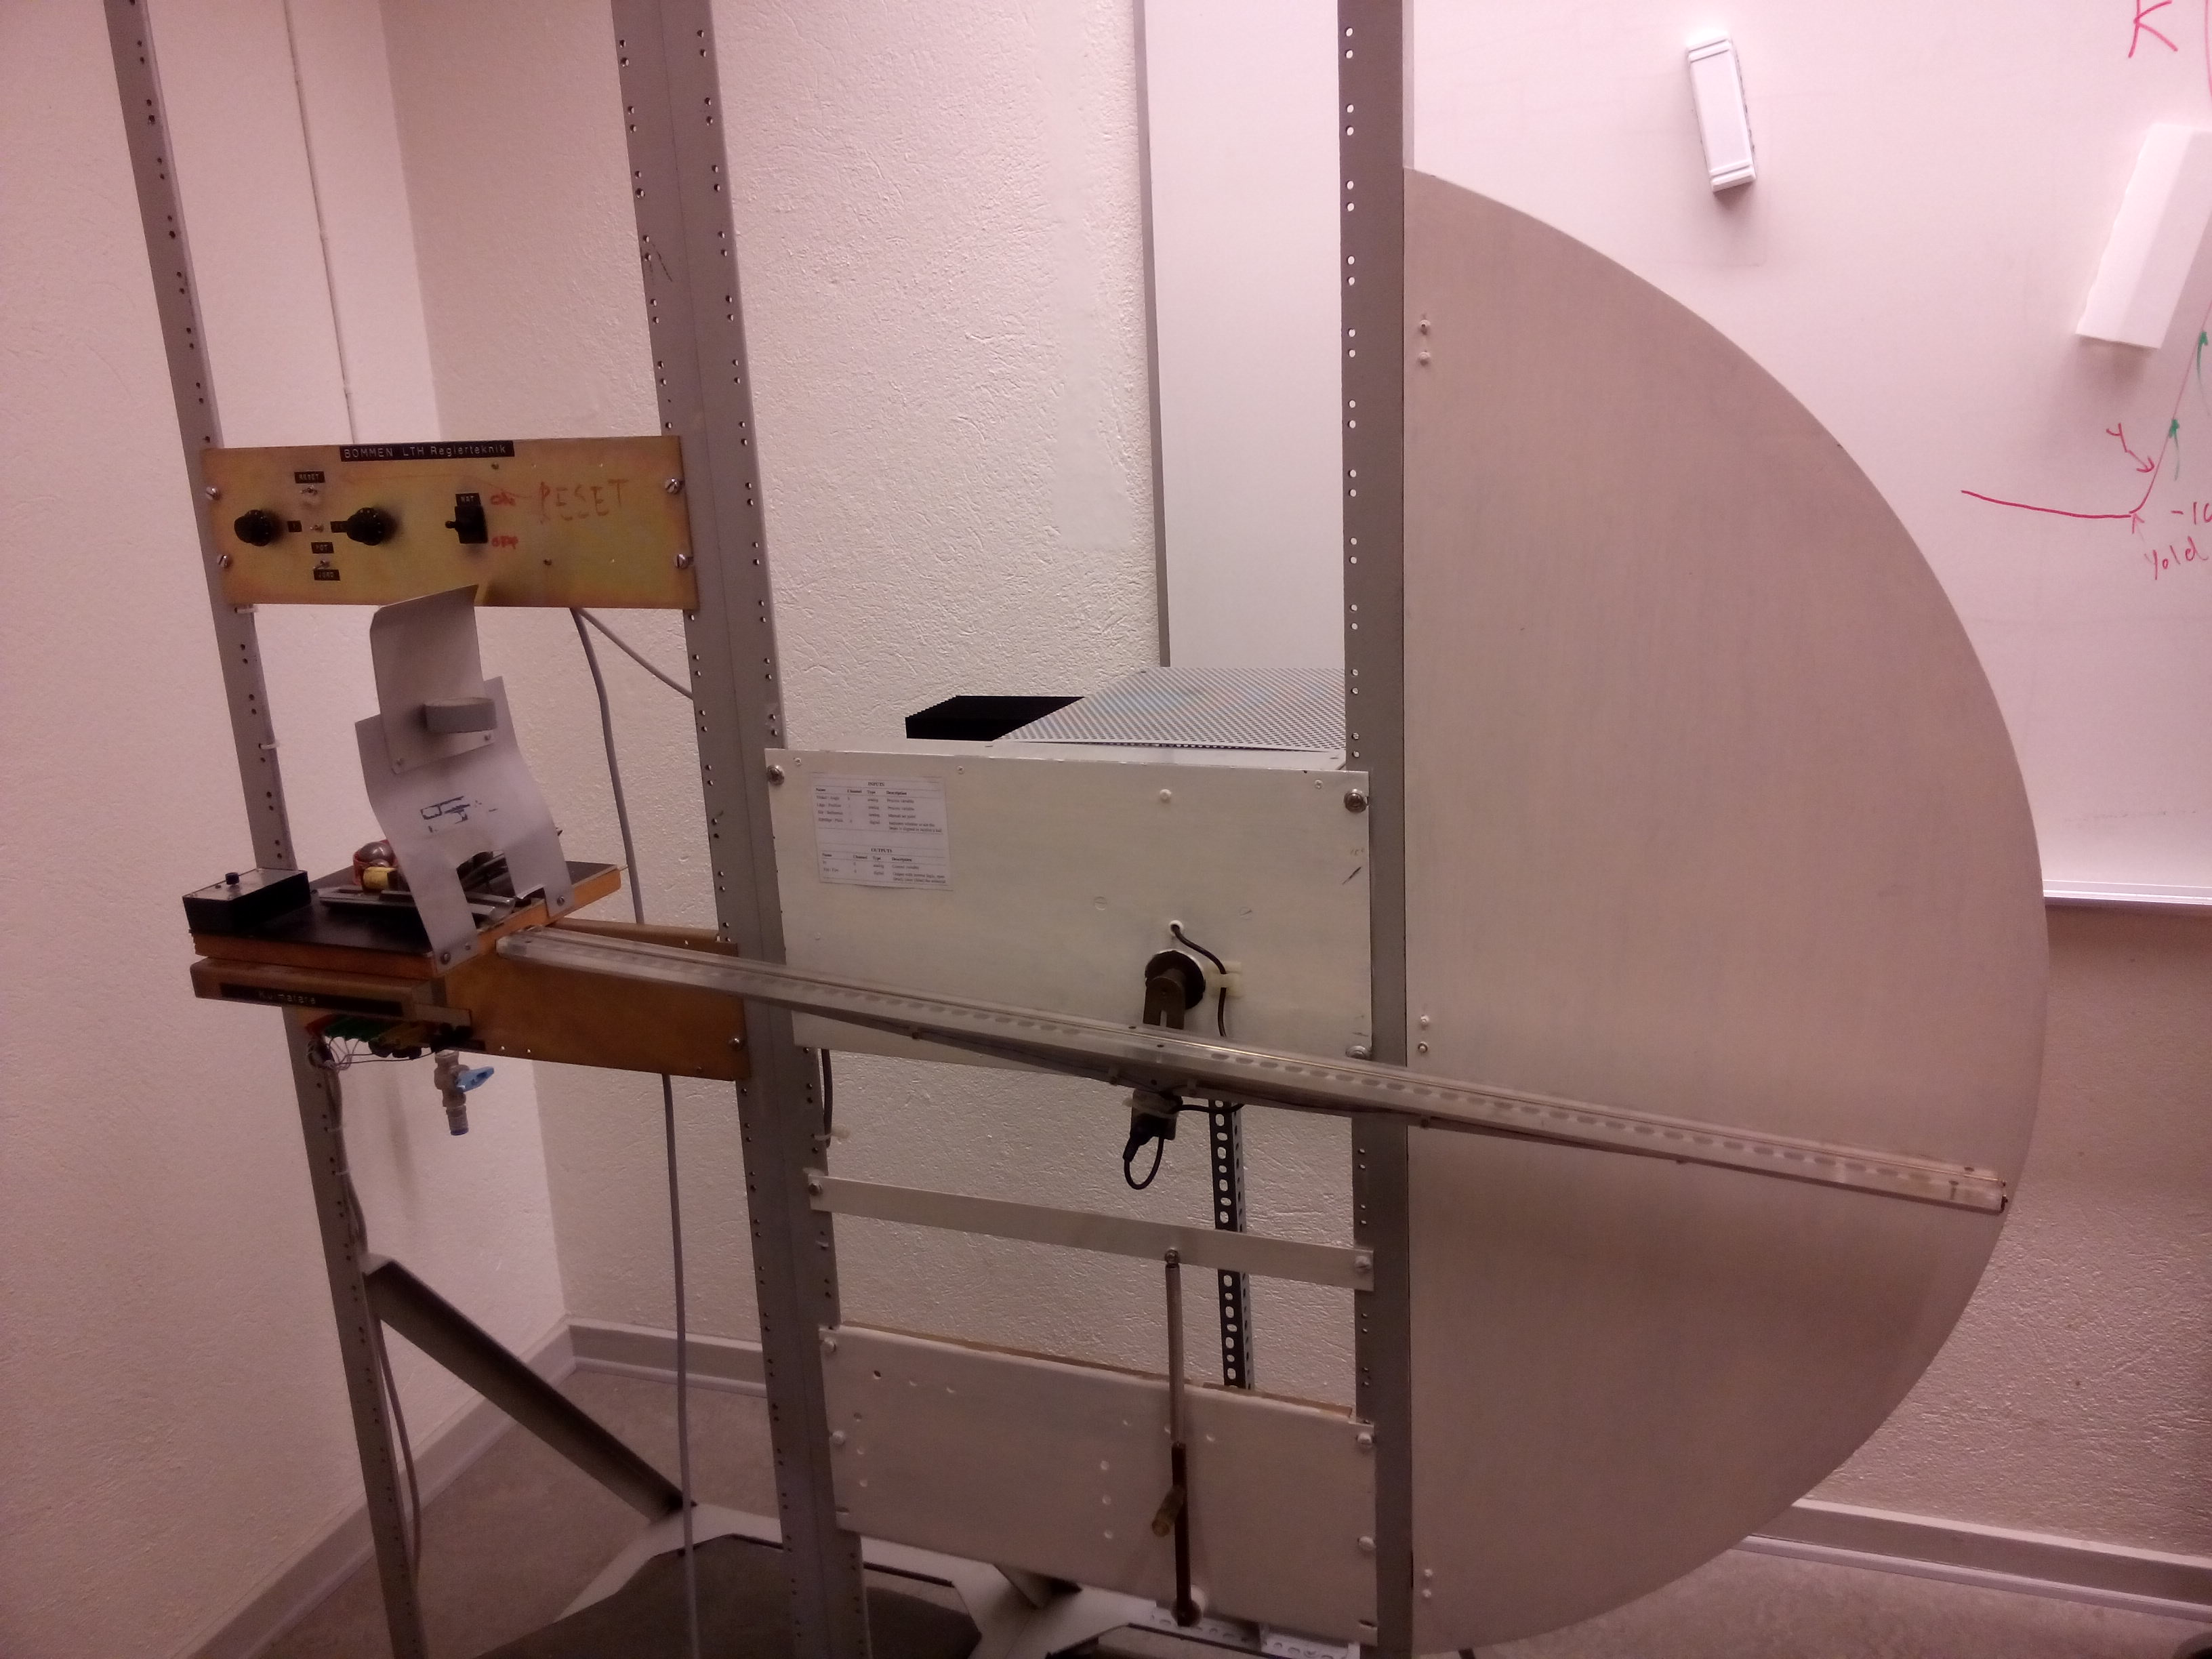
\includegraphics[width=0.8\textwidth]{figures/process_fig.jpg}
\end{frame}

\begin{frame}
\frametitle{Catch and weigh ball}
\centering
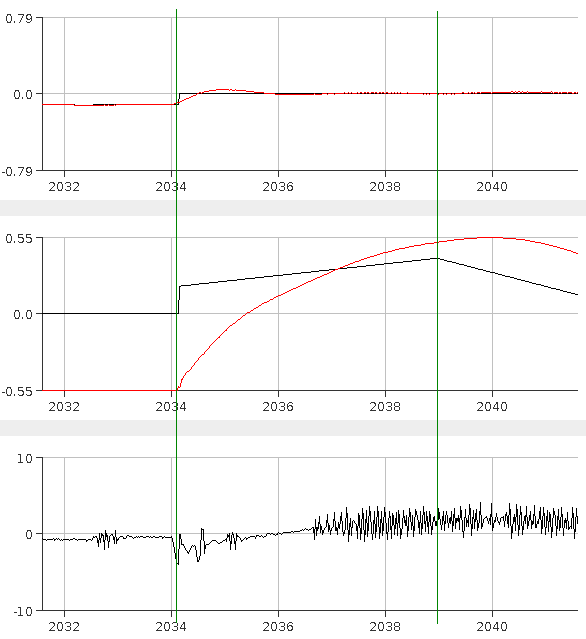
\includegraphics[height=0.83\textheight]{figures/weighmediumball-crop.png}
\end{frame}

\section{Program structure}
\frame{\sectionpage}
\begin{frame}
\frametitle{Class overview}

\end{frame}

\begin{frame}
\frametitle{RegulThread}

\end{frame}

\begin{frame}
\frametitle{SwitchThread}

\end{frame}

\section{Results and conclusions}
\frame{\sectionpage}
\begin{frame}
\frametitle{Step responses}
\centering
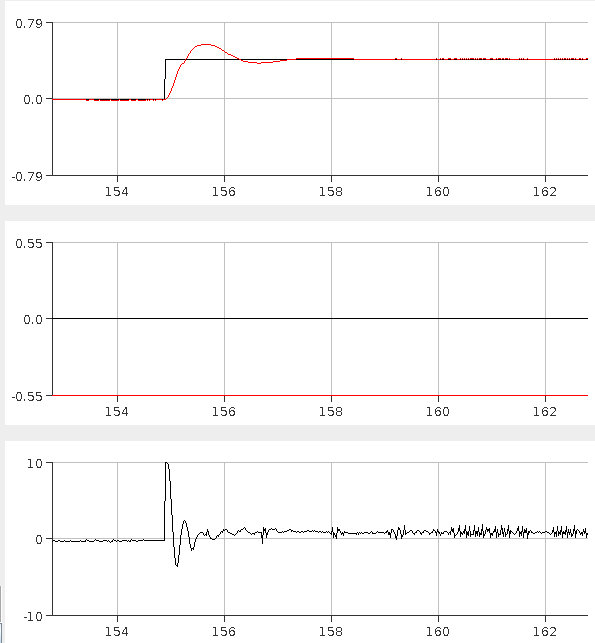
\includegraphics[width=0.45\textwidth]{figures/stepresponsebeam-crop.png}
\hspace{1em}
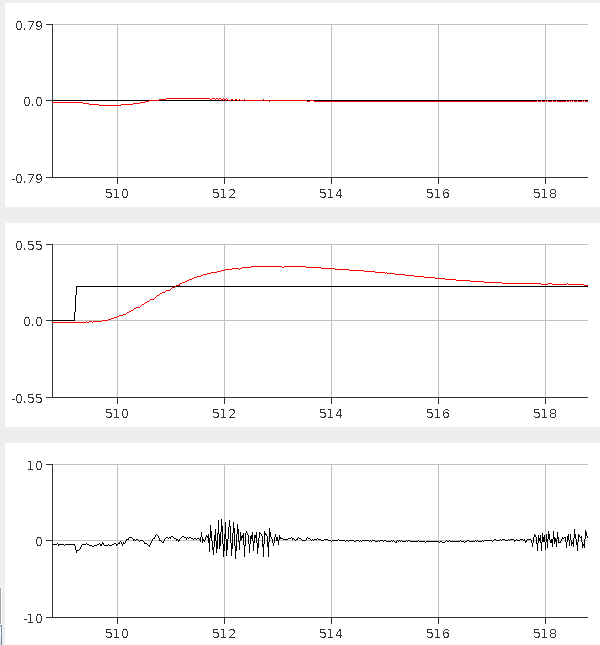
\includegraphics[width=0.45\textwidth]{figures/stepresponseball1-crop.png}
\end{frame}

\begin{frame}
\frametitle{Catching and weighing}
\centering
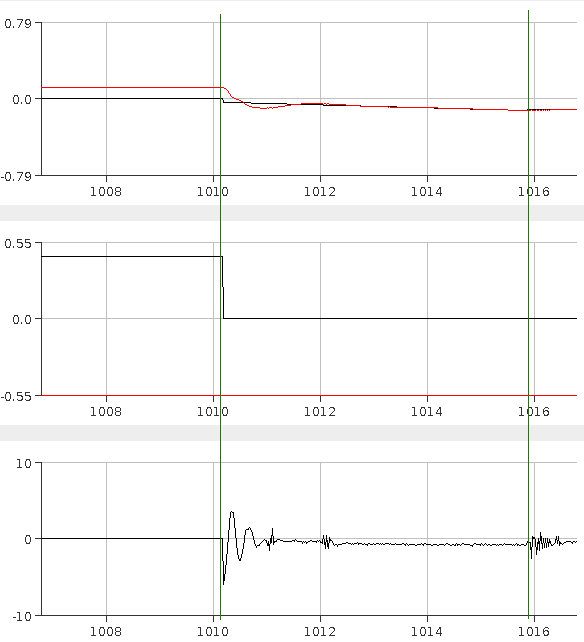
\includegraphics[width=0.45\textwidth]{figures/topickupposition-crop.png}
\hspace{1em}
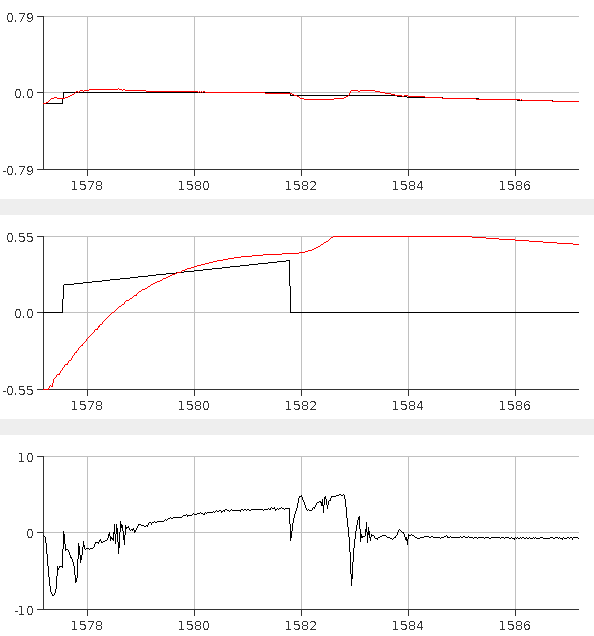
\includegraphics[width=0.45\textwidth]{figures/weighanddroplargeball-crop.png}
\end{frame}

\begin{frame}
\frametitle{Small and medium balls}
\centering
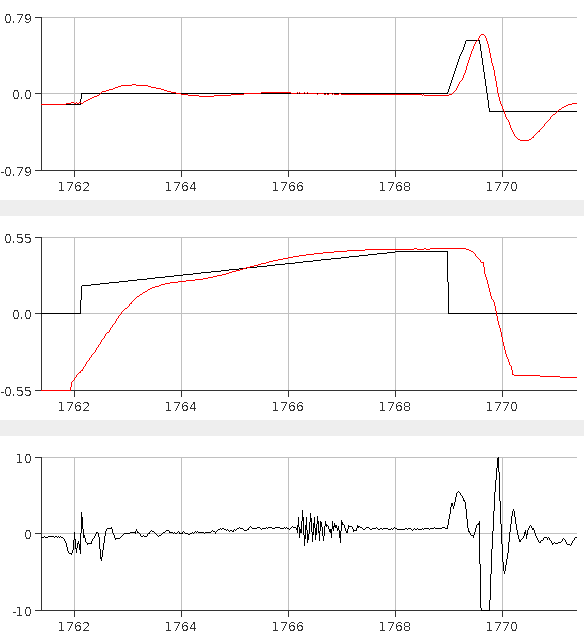
\includegraphics[width=0.45\textwidth]{figures/weighandthrowsmallball-crop.png}
\hspace{1em}
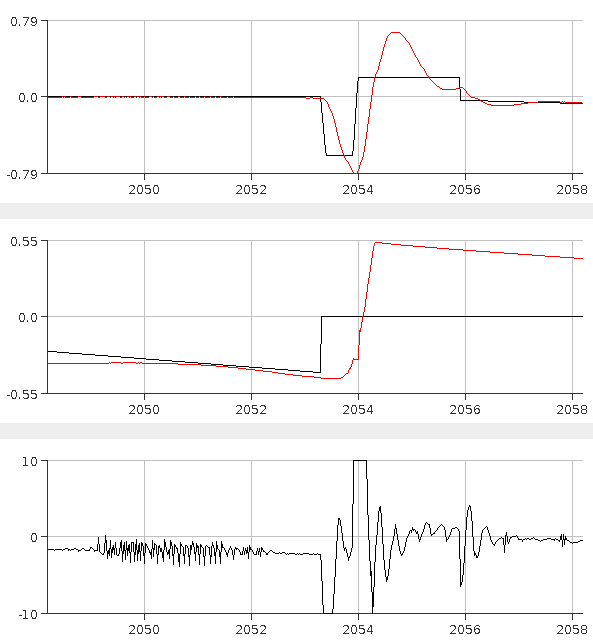
\includegraphics[width=0.45\textwidth]{figures/throwmediumball-crop.png}
\end{frame}

\begin{frame}
\frametitle{Numerical optimization approach}
\centering
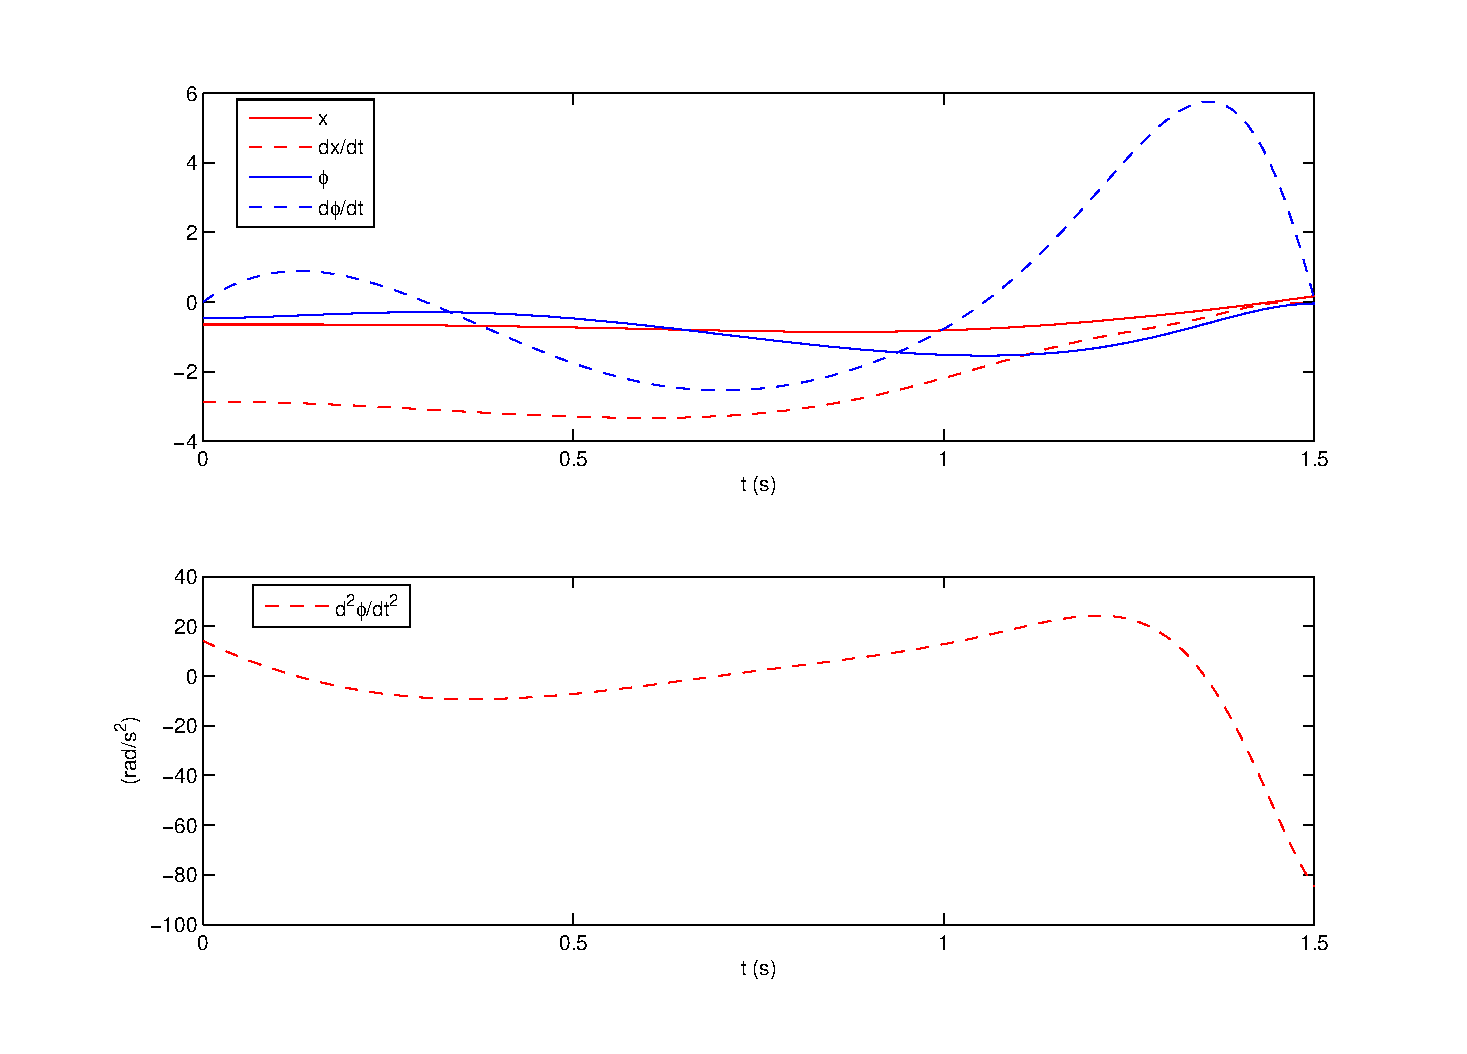
\includegraphics[width=0.9\textwidth]{ballbeammatlab.eps}
\end{frame}


%\section{Beamer}
%
%\frame{\tableofcontents[current]}
%
%\subsection{Demo}
%
%\begin{frame}
%\frametitle{Magic!}
%\uncover<2->{One can display and remove objects on the same slide:}
%\begin{overlayarea}{\textwidth}{6cm}
%\begin{itemize}
%\item<3-> \uncover<3->{{\color{structure}Words in disarray.}}
%\only<4-8>{\newline \uncover<8->{That} \uncover<7->{phrase} \uncover<6->{appears} \uncover<5->{backwards} \uncover<4->{!}}
%\item<9-> \uncover<9->{{\color{structure}Words that replace others.}}
%\only<10-12>{\newline \only<10>{Blabla \dots}\only<11>{\dots\ blablabla \dots}\only<12>{\dots\ blablabli, \dots}}
%\item<13-> \uncover<13->{{\color{structure}A Table.}}
%\only<14-19>{
%\begin{center}
%\begin{tabular}{|c|c|c|}
%\hline
%\uncover<17->{AAA} & \uncover<19->{BBBB} & \uncover<15->{CCC} \\
%\hline
%\uncover<14->{$\mathbb D$} & \uncover<16->{$\mathbb R$} & \uncover<18->{$\mathbb F$}\\
%\hline
%\end{tabular}
%\end{center}
%}
%\item<20-> \uncover<20->{{\color{structure}And many other things!}}
%\begin{itemize}
%\item<21->{several columns;}
%\item<22->{fixed size zones;}
%\item<23->{print or handout versions;}
%% v \item<24->{transitions;}
%\item<24->{hyperlinks;}
%\item<25->{supplementary slides for questions;}
%%\item<27->{works with \texttt{latex} as well as with \texttt{pdflatex}.}
%\end{itemize}
%\end{itemize}
%\end{overlayarea}
%\end{frame}
%
%\begin{frame}
%% Transition pour ce transparent, 
%% la seule utilisÈe dans cette prÈsentation !
%\transsplithorizontalout<1>
%\frametitle{Maths with style}
%Maths formula can also be dynamical!
%
%\uncover<2->{A step by step computation\dots}
%\begin{align*}
%\uncover<3->{\langle d\omega, \sigma \rangle} &
%\uncover<5->{\alert<5>{\ = \int_{\Delta_p} \sigma^\ast d\omega}}
%\uncover<7->{\alert<7>{\ = \int_{\Delta_p} d( \sigma^\ast \omega)}} \\
% & \uncover<9->{\alert<9>{\ = \int_{\partial \Delta_p} \sigma^\ast \omega}}
% \uncover<10->{\alert<10>{\ = \sum_{i=0}^p (-1)^i \int_{\Delta_{p-1}} F^{p\ \ast}_i \sigma^\ast \omega}}\\ 
% & \uncover<10->{\alert<10>{\ =}} \uncover<8->{\ \alert<8>{\sum_{i=0}^p (-1)^i \int_{\Delta_{p-1}} (\sigma \circ F^p_i)^\ast \omega = }}
% \uncover<6->{\alert<6>{\int_{\Delta_{p-1}} (\partial \sigma )^\ast \omega}} \\
% & \uncover<4->{= \langle \omega, \partial \sigma \rangle}
%\end{align*}
%\end{frame}
%
%\subsection{Fractional Derivatives}
%
%\begin{frame}{Fractional Derivatives}
%$F$ is the Fourier Transform
%$$F\circ D^n = (i2\pi\xi)^n F$$
%$\alt<2>{\alpha }{n}$
%\begin{equation*}
%D^{\alt<2>{\alpha}{n}} f
%{(i2\pi k)^{\alt<2>{\alpha}{n}}}
% (i2\pi k)^{\alt<2>{\alpha}{n}} F f
%\end{equation*}
%\uncover<2>{$$(i2\pi k)^{\alpha} =  {|2\pi k|}^{\alpha} \exp\left(i\frac{\pi}{2}\alpha\mathrm{sgn}(k)\right)$$}
%\end{frame}
%
%
%\subsection{Documentation}
%\begin{frame}{Documentation}
%Make sure to read the excellent documentation for beamer:
%
%\url{http://www.ctan.org/tex-archive/macros/latex/contrib/beamer/doc/beameruserguide.pdf}
%\end{frame}
%
%\begin{frame}{Columns}
%You may divide the page in columns and/or blocks as follows:
%\begin{columns}
%\begin{column}{.4\textwidth}
%\begin{block}{Left}
%Left column.
%\end{block}
%\end{column}
%\begin{column}{.4\textwidth}
%\begin{block}{Right}
%Right column.
%\end{block}
%\end{column}
%\end{columns}
%\end{frame}
%
%\begin{frame}[fragile]{Fragile frames}
%If you have some verbatim text in the page \emph{make sure to use the fragile option.}
%\begin{verbatim}
%def some_function(arg):
%  print arg
%\end{verbatim}
%\pause
%(Note that you should use syntax highlighting for the example above.)
%\end{frame}
%
%\begin{frame}[fragile]{Graphic inclusion}
%To include graphics, you should simply use \verb|includegraphics| as usual:
%\begin{center}
%
\includegraphics[height=0.7\textheight]{logoonly}
%\end{center}
%\end{frame}
%
%\part{References}
%\frame{\partpage}
%
%\begin{frame}
%\frametitle<presentation>{References}  
%  \begin{thebibliography}{10}
%  \beamertemplatearticlebibitems
%  \bibitem{vonNeumann-self-adjoint}
%    A.~Devinatz and A.~E.~Nussbaum and J.~von~Neumann
%    \newblock On the permutability of self-adjoint operators.
%    \newblock {\em Ann. of Math.} (2) {\bf 62} (1955). 199--203
%    \pause
%  \bibitem{vonNeumann-matrices}
%    H.~H.~Goldstine and J.~von~Neumann
%    \newblock Numerical inverting of matrices of high order.
%    \newblock {\em Proc. Amer. Math. Soc.}, {\bf 2} (1951). 188--202
%\pause
%  \end{thebibliography}
%\end{frame}


\end{document}

